%for slideshow
\documentclass[ignorenonframetext]{beamer} %add option 'draft' for quicker compilation
\usepackage{beamerthemesplit}
\newcommand{\slides}{1}
%\includeonlyframes{current} %this only compiles frames with [label=current]
 
%for handouts
%\documentclass[a4paper,12pt]{article}
%\usepackage{beamerarticle}
%\newcommand{\slides}{0}

\mode<presentation>
{
%    \usetheme{AnnArbor}
  \usetheme{Darmstadt}
  \usecolortheme{seahorse}
  \setbeamercovered{transparent}
  %Add university logo
  \pgfdeclareimage[height=1cm]{university-logo}{logo}
  \logo{\pgfuseimage{university-logo}}
  % If you wish to uncover everything in a step-wise fashion, uncomment
  % the following command:
  \beamerdefaultoverlayspecification{<+->}
	\newcommand{\tcr}{\textcolor{red}}
}
\mode<article>{
 \usepackage{fullpage}
	\newcommand{\tcr}{\textcolor{black}}
  \renewcommand{\baselinestretch}{1.0}
  \oddsidemargin -1.5cm \evensidemargin -1.5in
  \topmargin=-1.5cm \headheight=0pt
  \headsep 0pt \textwidth=19cm
  \textheight=27cm \columnsep 10pt \columnseprule 0pt \parindent 0pt
  \parskip 0.0pt
  %\usepackage{tweaklist}
  %\renewcommand{\itemhook}{
  %  \setlength{\topsep}{-0pt}
  %  \setlength{\itemsep}{-0pt}
  %  \setlength{\parsep}{-0pt}
  %}
  %\renewcommand{\enumhook}{
  %  \setlength{\topsep}{-0pt}
  %  \setlength{\itemsep}{-0pt}
  %  \setlength{\parsep}{-0pt}
  %}
}

\usepackage[english]{babel}
\usepackage[latin1]{inputenc}
\usepackage{times}
\usepackage[T1]{fontenc}
\usepackage{epsf,graphics,graphicx,fancyhdr,color,amsmath,url,enumerate,alltt}
\usepackage{ifthen}

\newcommand{\bc}{\begin{center}}
\newcommand{\ec}{\end{center}}
\newcommand{\bn}{\begin{enumerate}}
\newcommand{\en}{\end{enumerate}}
\newcommand{\bi}{\begin{itemize}}
\newcommand{\ei}{\end{itemize}}
\newcommand{\be}{\begin{eqnarray}}
\newcommand{\ee}{\end{eqnarray}}
\newcommand{\bes}{\begin{eqnarray*}}
\newcommand{\ees}{\end{eqnarray*}}

\title[MT4113]{MT 4113: Computing in Statistics}

\subtitle{Computer intensive statistics\\Lecture 6: Permutation, randomization, and Monte-Carlo tests}

\author[Lecture 6]{Len Thomas}

%\institute{School of Mathematics and Statistics, University of St Andrews}

\date[10/10/2018] {Oct 10  2018}

% Delete this, if you do not want the table of contents to pop up at
% the beginning of each subsection:
\mode<presentation> {
    \AtBeginSubsection[]
    {
    \begin{frame}<beamer>
        \frametitle{Outline}
        \tableofcontents[currentsection,currentsubsection]
    \end{frame}
    }
}
\begin{document}

\begin{frame}
  \titlepage
\end{frame}

\mode<article>{
\maketitle
}

\mode<presentation> {
\begin{frame}
  \frametitle{Outline}
	\tableofcontents
  % You might wish to add the option [pausesections]
\end{frame}
}

\section{Introduction}

\subsection{Revision -- Traditional parametric and nonparametric methods}

\begin{frame}
	\frametitle{Problem statement -- inference from one sample}
	\bi
		\item We have a sample of data $x = x_1, \ldots, x_n$ that are realizations of iid random variables $X=X_1, \ldots, X_n$ with pdf $f()$.
		\item We wish to make inferences about some population characteristic -- say the mean $\mu$ of $f()$.
	\ei
\end{frame}

\begin{frame}
	\frametitle{Parametric methods}
	\bi
		\item Assume $f()$ is a known function with parameters $\theta$ -- e.g., $f(\theta)=\mbox{N}(\mu,\sigma^2)$.
		\item For a (two-sided) hypothesis test
		\bi
		  \item Specify the null hypothesis, $H_0$ -- e.g., $\mu=\mu_0$
			\item Construct a test statistic $T(X)$ that has a known distribution under $H_0$
			\item e.g.,
			\begin{equation*}
			    T(x) = \frac{\bar{x}-\mu_0}{s/\sqrt{n}}
			\end{equation*}
			which has a $t$-distribution with mean 0, variance 1 and $\mbox{d.f.}=n-1$, if $H_0$ is true
			\item Calculate $P(\left|T(X)\right| \geq \left|T(x)\right|;\mu_0)$ -- the $p$-value.
			\item If $p\mbox{-value} \leq \alpha$ the result is statistically significant.
%Note - At this point I typically draw a picture of a t-distribution with mean 0 and variance 1, and show how the df influences the heaviness of the tails.  I then draw on a T(x) for some x and shade in the more extreme parts to show this is the p value.  (Can mention how bigger variance also makes the T(x) smaller.)
%There's a photo of such a figure in the lecture directory
		\ei
	\ei
\end{frame}
\begin{frame}
	\ifthenelse{\slides=1}{\frametitle{Parametric methods (contd.)}}{}
	\bi
		\item For (two-sided) confidence intervals on $\mu$
		\bi
			\item For $((1-\alpha)\times 100) \%$ limits, find the scalar values $L(X)$ and $U(X)$ such that
			\begin{equation*}
			    P\left(L(X)<\mu \mbox{\ and\ } U(X)>\mu\right) = 1-\alpha
			\end{equation*}
			\item Many methods for finding the limits
			\item E.g., inverting the test statistic
			\bi
				\item limits are the smallest and largest values of $\mu_0$ that are not rejected under $H_0: \mu=\mu_0$
%At this point, I could draw a line and note on it barx, and then below some mu0 and an arrow down to text that says L(X) is the value of mu0 where P(T(X)>=T(x))=alpha/2, and then show the distribution of t above it and the tail probability; then could do the same for U(X) -- there's a photo of a figure to draw in the lecture directory
				\item E.g., $t$-based intervals  $\bar{x} \pm t_{\alpha/2,n-1} s /\sqrt{n}$
%Can say in the case of a t-distribution it turns out these are symmetric about barx - at distance t_{alpha/2,n-1} s/sqrt(n) above and below.
			\ei
		\ei
    \item So, for parametric methods, you need to specify two distributions:
			\bi
				\item The pdf generating the data: $f(\theta)$
				\item The distribution of the test statistic: $T(X)$
		  \ei
	\ei
\end{frame}

\begin{frame}
	\frametitle{Traditional nonparametric methods}
	\bi
		\item Avoid fully specifying the distribution of $f()$.
		\item E.g., Wilcoxon signed ranks test
		\bi
		  \item $f()$ is symmetric about some median m
		  \item $H_0: m=m_0$
		  \item Test statistic
			\begin{equation*}
			    	T(x)=\sum_{i:x_i\neq{m_0}} \mbox{rank}(|x_i-m_0|) \mbox{sign}(x_i-m_0)
			\end{equation*}
      where $\mbox{rank}(x)$ denotes the rank order of $x$ (smallest has value 1, next smallest 2, etc.) and $\mbox{sign}(x-y)$ is a sign function, having value 1 if $x>y$ and -1 if $x<y$.
%Can take the time to explain this, perhaps with a small example.  Numbers 2, 3.5, 5, 7, 9 and median 5.  Show that you calculate the differences, assign them ranks (smallest gets rank 0) and signs and add up the rank plus sign.		
			\item Under $H_0$, T(X) has (approximately) a normal distribution
			\item For confidence limits on $m$, can invert the test statistic
	
		\ei
	\ei
\end{frame}

\begin{frame}
	\frametitle{Computer-intensive statistical methods}
	\bi
		\item With computer intensive methods, you can avoid the need to fully specify either the distribution of $f()$ and/or $T(X)$
		\item Examples:
		\bi
			\item Permutation-based approach to Wilcoxon test\\
			(avoids the need to specify distribution for $T(X)$; Wilcoxon already avoids $f()$)
			\item Monte-Carlo-based version of the $t$-test\\
			(avoids specification of $T(X)$, but not $f(\theta)$)
			\item Parametric and non-parametric bootstrap confidence intervals\\
			(again avoids $T(X)$; either specify or not $f(\theta)$)
		\ei
	\ei

\end{frame}

\subsection{Motivating example}

\begin{frame}
	\frametitle{Pine martin habitat preference data}
\bc
\includegraphics[height=1.8in]{pine_martin}
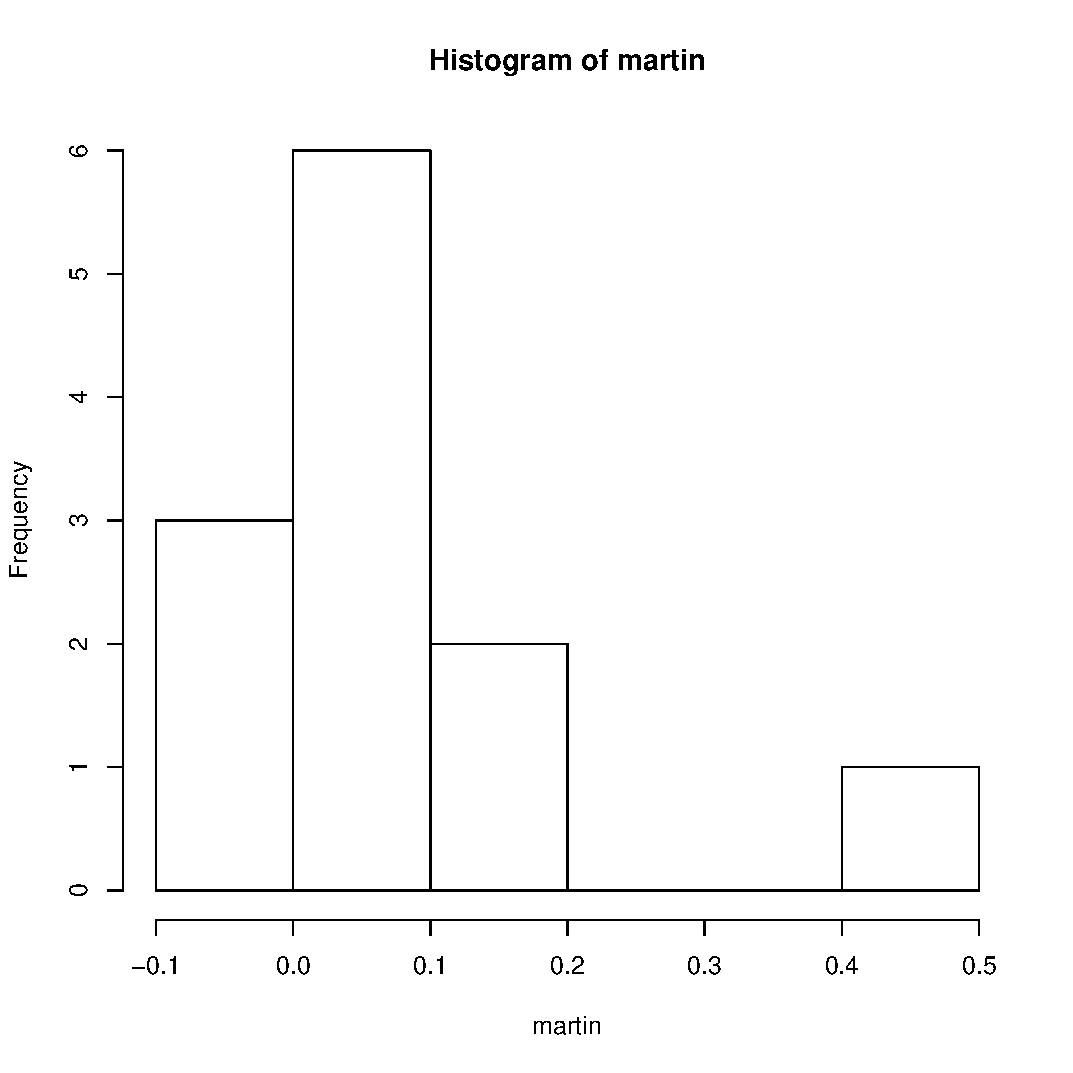
\includegraphics[height=1.8in]{martin_hist}
\ec
	\bi
		\item 0.13, -0.01, -0.01, 0.42, -0.02, 0.01, 0.09, 0.03, 0.04, 0.06, 0.12, 0.03
		\item Shapiro-Wilk test for normality W = 0.70, p<0.001
	\ei
\end{frame}

\begin{frame}
	\frametitle{Pine martin example: parametric test}
	\bi
		\item Assume data come from a normal distribution
			\bi
				\item $H_0: \mu=0$
				\item $t$-test: $t=2.147$, d.f.=11, $p=0.055$
				\item $\bar{x}=0.074$, 95\% $t$-based CI: (-0.002, 0.150) 
			\ei
		\item Could try transforming -- e.g., $\mbox{log}(x_i + 0.03)$:\\
\bc
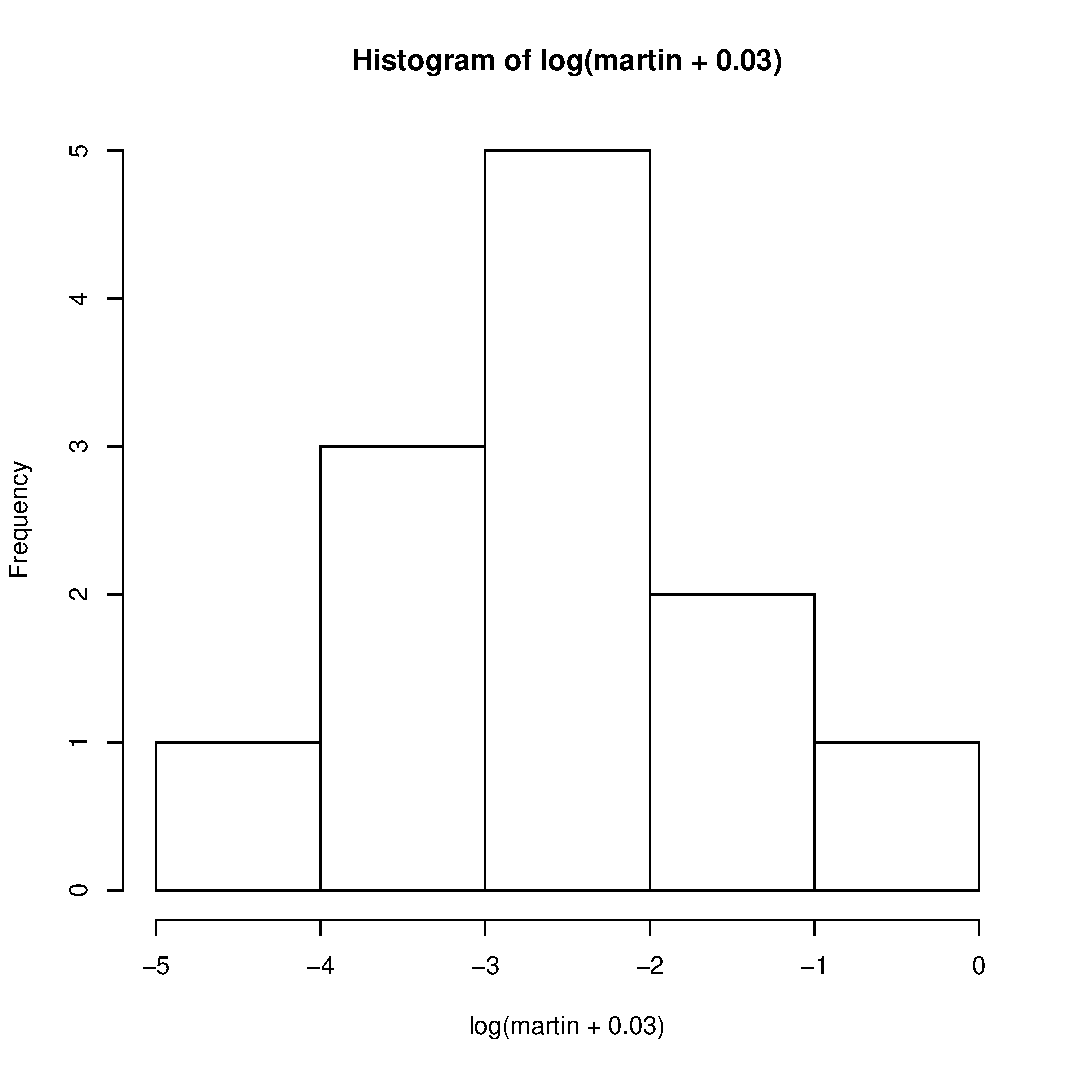
\includegraphics[height=1in]{martin_hist_log}
\ec
		\bi
			\item $H_0: \mbox{log}(\mu+0.03)=\mbox{log}(0.03)$
			\item $t$-test: $t=2.484$, d.f.=11, $p=0.030$
			\item 95\% $t$-based CI (back-transformed): (0.003, 0.095) 
		\ei
	\ei
\end{frame}
\begin{frame}
	\frametitle{Pine martin example: parametric test (contd.)}
	\bi
    \item Problems:
    \bi
			\item Result not invariant to transformation: what transformation to use?
			\item If we use log, then what about bias correction?
    \ei					
	\ei
\end{frame}

\begin{frame}
	\frametitle{Pine martin example: traditional nonparametric test}
	\bi
		\item Wilcoxon signed-ranks test:
		\bi
			\item $H_0: m=0$
			\item $p = 0.012$
			\item 95\% CI on m: (0.010, 0.120)
		\ei
		\item Disadvantages:
		\bi
			\item Requires us to formulate $H_0$ in terms of the median
			\item Less powerful than a $t$-test when parametric assumptions met
		\ei	
	\ei
\end{frame}

\section{Permutation methods}

\subsection{Permutation test}

\begin{frame}
	\frametitle{Pine martin example}
	\bi
		\item Under $H_0: \mu=\mu_0$, and assuming the distribution of $x_i$ is symmetric about $\mu_0$, then
		\item $+(x_i - \mu_0)$ is just as likely to occur in the data as $-(x_i - \mu_0)$
		\item For $\mu_0=0$ then $+x_i$ is just as likely as $-x_i$
		\item So, can produce alternative equally likely realizations of the data by swapping any $x_i$ for $-x_i$
	\ei
\end{frame}

\begin{frame}
	\frametitle{Permutations}
	\bi
		\item <1->Given 12 data points, there are $2^{12}=4096$ ways to do this:
    \bi
			\item <2->0.13, 0.01, 0.01, 0.42, 0.02, 0.01, 0.09, 0.03, 0.04, 0.06, 0.12, 0.03		
			\item <2->-0.13, 0.01, 0.01, 0.42, 0.02, 0.01, 0.09, 0.03, 0.04, 0.06, 0.12, 0.03		
 			\item <2->0.13, -0.01, 0.01, 0.42, 0.02, 0.01, 0.09, 0.03, 0.04, 0.06, 0.12, 0.03		
 			\item <2->0.13, 0.01, -0.01, 0.42, 0.02, 0.01, 0.09, 0.03, 0.04, 0.06, 0.12, 0.03		
			\item <2-> $\vdots$
 			\item <2->-0.13, -0.01, -0.01, -0.42, -0.02, -0.01, -0.09, -0.03, -0.04, -0.06, -0.12, -0.03	     \ei
	\ei
\end{frame}

\begin{frame}
	\frametitle{Permutation test}
	\bi
		\item<1-> Find what proportion of the permutations have $|\bar{X}|$ greater than the observed $|\bar{x}|$.
\visible<2->{\bc
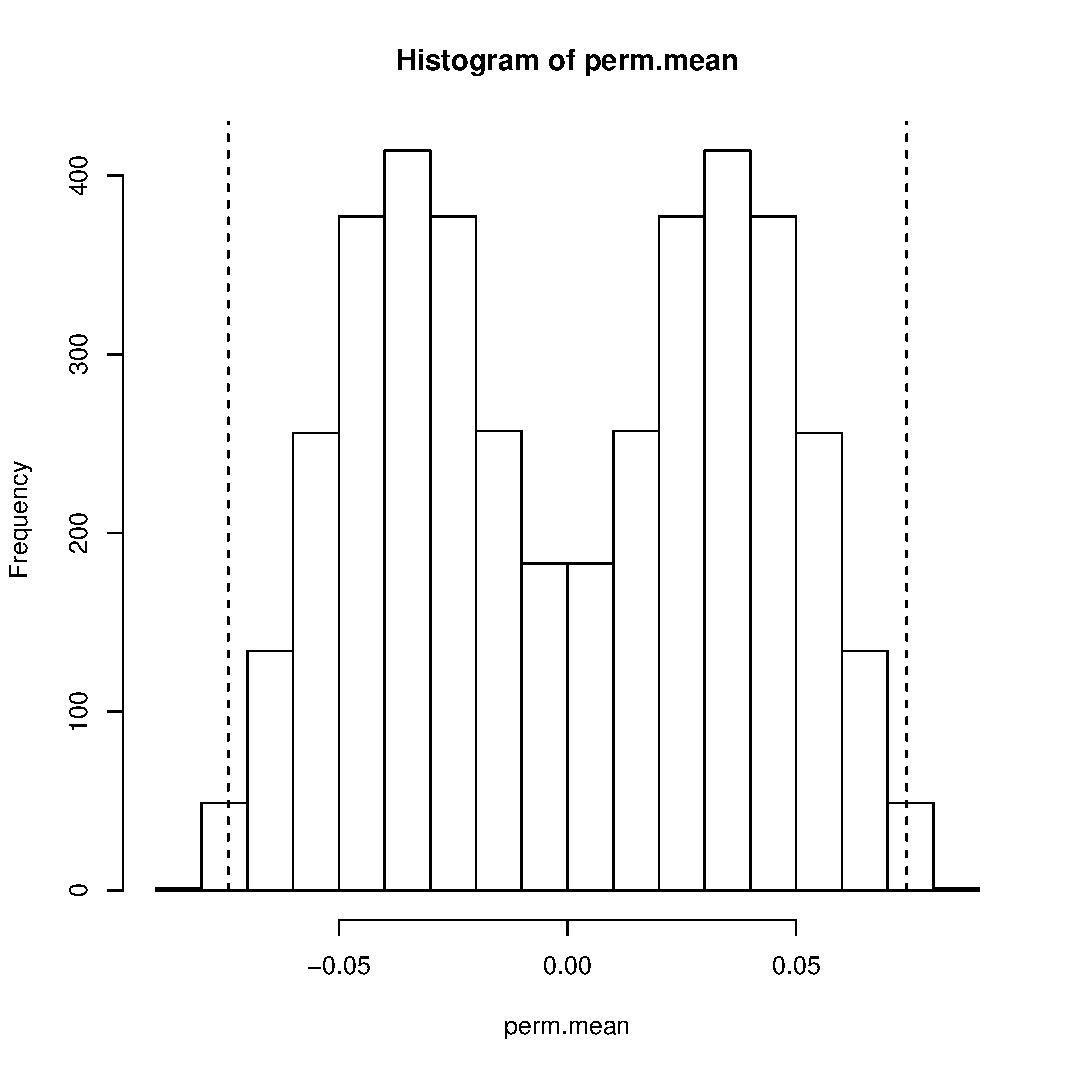
\includegraphics[height=1.9in]{perm}
\ec}
		\item<2-> 48 out of 4096 are as extreme - so $p=48/4096=0.012$
	\ei
\end{frame}

\begin{frame}
	\frametitle{Permuatation tests - the basic idea}
	\bi
		\item Pick a null hypothesis $H_0$ and test statistic $T(X)$
		\item Under $H_0$, all possible appropriate data permutations (re-orderings) are equally likely
		\item So, calculate $T(X)$ for each permutation and see how extreme $T(x)$ is compared with these
			\bi
		  \item If $T(x)$ is extreme, reject $H_0$
		  \item If $T(x)$ is not extreme, don't reject $H_0$
		  \ei
  \ei
 No need to specify distributions for:
  \bi
		\item $f()$ - no parametric definition needed
		\item $T(X)$ - obtain this via the randomization procedure
	\ei
\end{frame}

\begin{frame}
	\frametitle{Choice of test statistic}
	\bi
		\item With permutation-based methods (and many other computer-intensive methods) you are free to choose whatever test statistic you like
		\item For example, we could use the median, trimmed mean, $t$-statistic, etc., etc.
		\item The method readily extends to other situations -- e.g., two sample tests, ANOVA, etc., etc.
	\ei
\end{frame}

\subsection{Permutation interval}

\begin{frame}
	\frametitle{Permutation interval}
	\bi
		\item Invert the test statistic: \\
		      Find the set of values of $\mu_0$ such that $H_0: \mu=\mu_0$ is not rejected
		\item For each potential value of $\mu_0$, follow the same procedure as before 
		\bi
		  \item calculating all permutations of $\pm (x_i - \mu_0)$
		  \item then seeing how extreme the observed $\bar{x}$ is among the permutations
		\ei
		\item Can use stochastic search methods\footnote{e.g., Robbins-Monroe search - see accompanying notes} to find the confidence limits
		\item In our example, 95\% CI is (0.013, 0.150) (c.f., $t$-based CI of (-0.002, 0.150)).
	\ei
\end{frame}

\subsection{Summary}

\begin{frame}
	\frametitle{Pros}
	\bi
		\item Widely applicable
		\item Produces exact results
		\item No specific distribution assumed for the data
		\item Does not require analytic distribution of test statistic
	\ei
\end{frame}

\begin{frame}
	\frametitle{Cons}
	\bi
		\item Each permutation of the data must be equally likely (or probability of occurrence is known)
		\item To be generally applicable, requires thought, and ability to program a computer (permutation algorithms
		      can be non-trivial)
		\item Can be prohibitively computer (and programmer) intensive in complex situations or for large sample sizes
	\ei
\end{frame}

\section{Randomization methods}

\subsection{Overview}

\begin{frame}
	\frametitle{Introduction}
	\bi
		\item Randomization methods are like permutation methods, except that a only random subset of all the possible permutations are generated
		\item E.g., pine martin example:
		\bi
			\item To generate one randomization, list the set of values $|x_i - \mu_0|$ and randomly assign a sign to each value
			\item From one run of 999 randomizations plus the original data value, I obtained $p=0.015$, very similar to the $p=0.012$ of the permutation method.
		\ei 
		\item Confidence intervals can be obtained in a similar way to permutation intervals
	\ei
\end{frame}

\subsection{Summary}

\begin{frame}
	\frametitle{Pros, compared with permutation methods}
	\bi
		\item All of the same advantages as permutation, plus
		\item Much easier to code
		\item Number of randomizations is fixed, rather than being a function of sample size
	\ei
\end{frame}

\begin{frame}
	\frametitle{Cons, compared with permutation methods}
	\bi
		\item As with permutation tests, each randomization of the data must be equally likely (or probability of occurrence is known)
		\item Results will vary from run to run
		\bi
			\item Size of this ``Monte-Carlo variation'' depends on the number of randomizations
		\ei
	\ei
\end{frame}

\section{Monte-Carlo tests}

\subsection{Overview}

\begin{frame}
	\frametitle{Introduction}
A generalization\footnote{If the assumed model for $f()$ implies that all data orderings are equally likely then you get back to a randomization test} of randomization tests to include parametric distributions for the data.
	\bi
		\item Algorithm:
		\begin{enumerate}
			\item Set up some distribution for the data, $f()$ or $f(\theta)$, and some $H_0$
			\item Repeat the following two steps many times:
			\begin{enumerate}
			  \item Simulate a data set according to $H_0$
			  \item Calculate $T(X)$ using the simulated data
			\end{enumerate}
			\item Add $T(x)$ evaluated from the sample data
			\item Order all of the $T(X)$s
			\item $p$-value is the proportion of the $T(X)$s as extreme or more extreme than the one from the sample data
		\end{enumerate}
	\ei

\end{frame}

\begin{frame}
	\frametitle{Pine martin example - parametric simulation}
	\bi
		\item <1->Assume observations are iid $\mbox{N}(\mu,\sigma^2)$, that $H_0: \mu=0$, and that $\sigma^2 = s^2$
		\item <2->Simulate 999 data sets of 12 observations from $\mbox{N}(0,s^2)$.
		\item <3->Calculate $\bar{x}$ for each of these, and add in the mean from the sample data, to give 1000 values of $\bar{x}$.
		\item <4->$p$-value is the proportion of these values that are more extreme (e.g., $p=0.029$)
\visible<4->{\bc
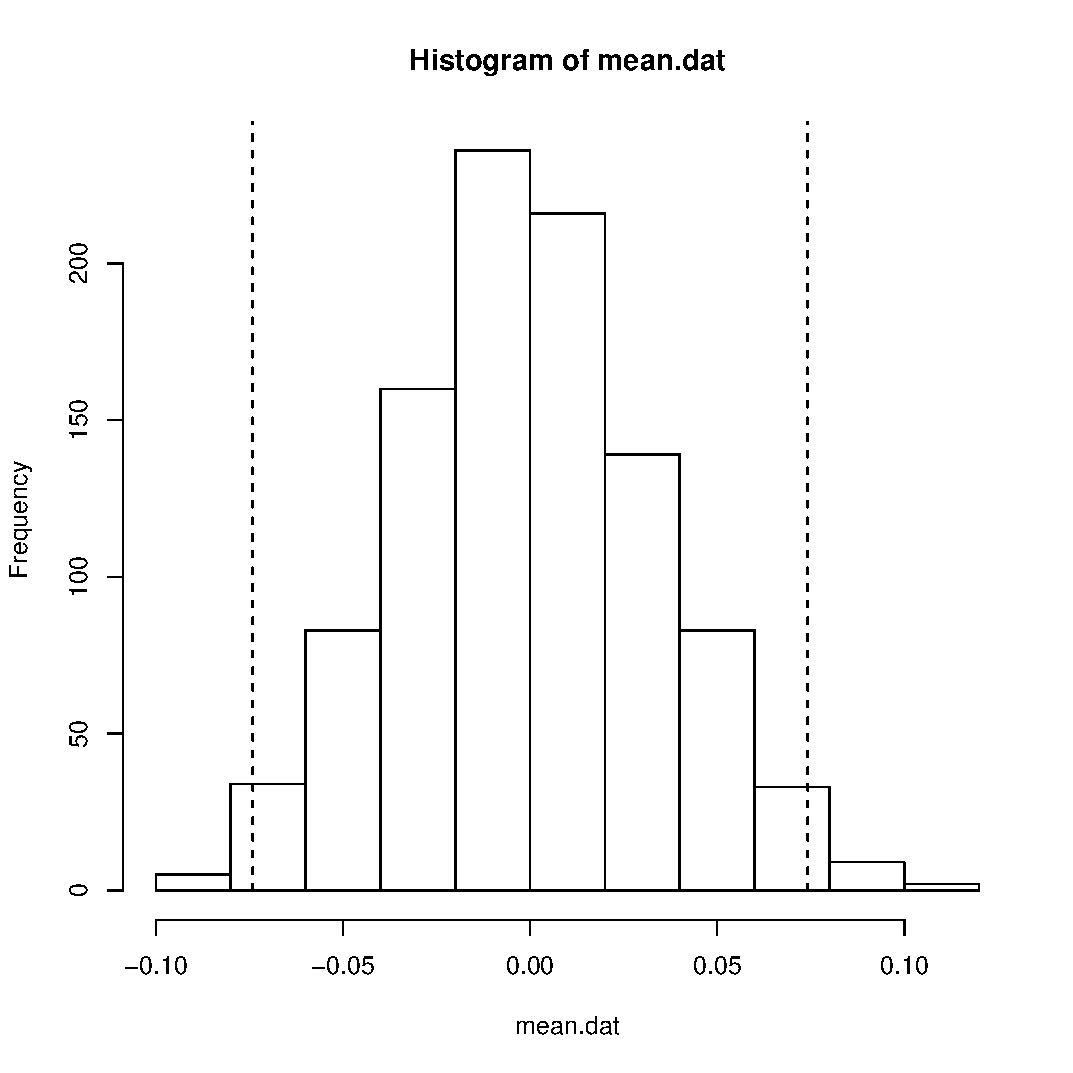
\includegraphics[height=1.2in]{mc}
\ec}
	\ei
\end{frame}

\subsection{Summary}

\begin{frame}
	\frametitle{Pros}
	\bi
		\item Data can be assumed to follow any distribution - parametric or non-parametric \\
		(Randomization tests are a special case)
		\item The analytic distribution of the test statistic is not required
	\ei
\end{frame}

\begin{frame}
	\frametitle{Cons, compared with permutation methods}
	\bi
		\item For parametric simulations, need to estimate nuisance parameters (e.g., $\sigma^2$ in the pine martin example)
		\item Results will vary from run to run
	\ei
\end{frame}

\begin{frame}
	\frametitle{Monte Carlo confidence intervals}
Confidence intervals can be constructed using similar methods to randomization intervals -- but there is a better way -- see next lecture...
\end{frame}

\end{document}


